\begin{figure*}[htb]
\centering
\subfigure[a] {\label{fig:ite}   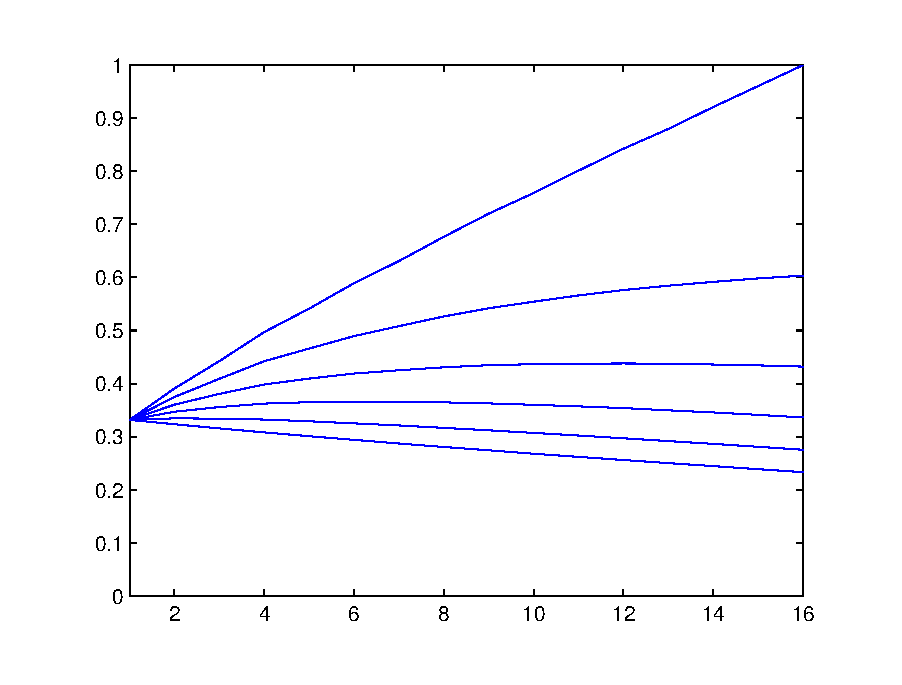
\includegraphics[width=0.32\textwidth]{fig/ppw_16_ite.eps}}
\subfigure[b] {\label{fig:taylor}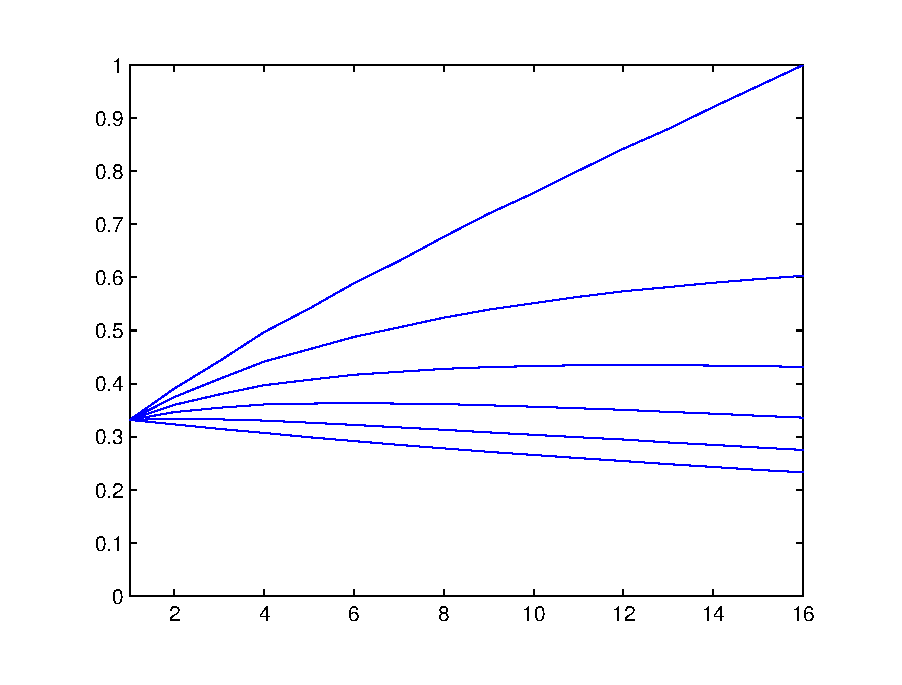
\includegraphics[width=0.32\textwidth]{fig/ppw_16_taylor.eps}}
\subfigure[c] {\label{fig:tayboo}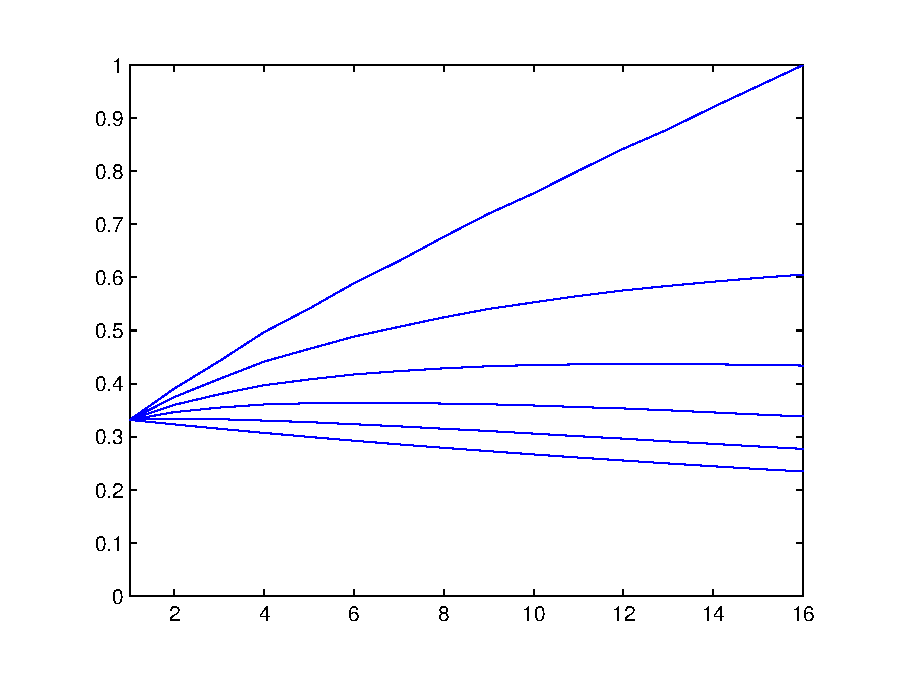
\includegraphics[width=0.32\textwidth]{fig/ppw_16_tayboo.eps}}
\caption{PPW}  
\label{fig:ppw}
\end{figure*}

\section{New Method}
This work aims to find the optimal number and distribution of active cores for a fixed set of cores to achieve the highest performance-per-watt, with consideration of thermal constraints. In order to estimate the power consumption of a multi-core chip for different number of active cores and various active core distributions, we first propose an iteration based full-chip power estimation method, which is accurate but very time-consuming. Furthermore, a non-iteration based method is proposed, which can implement local linearization to avoid time-consuming iterations. Additionally, a greedy based method can be integrated into the non-iteration based power estimation method to achieve further acceleration.

\subsection{Iteration based leakage-aware power estimation}
Because of the dependency of static power on temperature, it's not straightforward to compute the static power and temperature of next steady state based on current static power and temperature. Iteration method can be implemented to solve such problem, the computation flow is shown in Fig.x.

The initial value of $P^0_s(T,t+h)$ is a guess we provide based on the process technology. The temperature distribution $T(t+h)^0$ can be calculated with such guess. $P^1_s(T,t+h)$, the static power of next time step is updated with $T(t+h)^0$. Next, the temperature distribution $T(t+h)^1$ can be derived from $P^1_s(T,t+h)$, which concludes one iteration loop. Such iteration goes on until the convergence test is satisfied as $\parallel P^i_s(T,t+h)$-$P^(i-1)_s(T,t+h)\parallel<\epsilon$. Finally, the static power and temperature of steady state is outputted.

The iteration based method can produce an accurate outcome providing the $\epsilon$ is chosen to be small enough, yet the computing time is a serious problem, especially when the number of cores is large enough.

\subsection{Local linearized thermal model}
The major difficulty of calculating leakage-aware power estimation comes from the nonlinear thermal model shown in (x), which is caused by the nonlinear relation between subthreshold current and temperature.

To reduce the long computing time caused by iteration method, the leakage current $I_{leak}$ can be linearized to eliminate the non-linearity between $p_{s}$ and temperature, thus accelerating the computation.

Taylor expansion is performed on the original $I_{leak}$ model at a expansion point $T_{0}$. Thus the linearized relation of $I_{leak}$ and temperature is obtained as:
\begin{equation}\label{linear_subthreshold}
\begin{split}
I_{sub} = &K(\frac{k}{q})^{2}e^(\frac{q(V_{GS}-V{th})}{\eta kT_{p0}}\\
&\times (T_{p0}^{2}+(2T_{p0}-\frac{q(V_{GS}-V_{th})}{\eta k})(T_{p}-T_{p0}))\\
&+ o[(T_{p}-T_{p0})^{2}],
\end{split}
\end{equation}
where $o[(T_{p}-T_{p0})^{2}]$ is the remainder. By ignoring the remainder, the linearized $I_{sub}$, denoted as $I_{lin}$ can be expressed as:
\begin{equation}\label{linear_subthreshold}
\begin{split}
I_{lin} = &K(\frac{k}{q})^{2}e^(\frac{q(V_{GS}-V{th})}{\eta kT_{p0}}\\
&\times (T_{p0}^{2}+(2T_{p0}-\frac{q(V_{GS}-V_{th})}{\eta k})(T_{p}-T_{p0})).
\end{split}
\end{equation}

Provided the actual temperature value $T_{p}$ is close to the reference temperature point $T_{p0}$, the approximation accuracy of $I_{lin}$ can be guaranteed. From previous research, it has been shown that due to the characteristic of today's semiconductor process, such local linear approximation of leakage current has high accuracy around the expansion point.

With the linearized relation of subthreshold current and temperature, the relation between static power and temperature in linear form can also be achieved as:
\begin{equation}\label{linear_static}
\begin{split}
p_{s} &= V_{dd}I_{leak}\\
&= V_{dd} \times (I_{lin}+I_{gate})\\
&= V_{dd} \times (I_{lin}(T_{p})+I_{const})
\end{split}
\end{equation}


The linearized static power equation in matrix form is
\begin{equation}\label{linear_static_matrix}
P_{s} = P_{0}+A_{s}T
\end{equation}

\begin{equation}\label{gt=bp}
(G - B_{c}A_{s})T(t) + C\frac{dT(t)}{dt} = B_{c}(P_{d}(t) + P_{0})
\end{equation}
\subsection{Non-iteration based power estimation}
As a property of Taylor expansion approximation, it is accurate only when the actual temperature $T_{p}$ is close to the expansion point $T_{p0}$. To find a totally accurate outcome, $T_{p} = T_{p0}$ is necessary. However, such strategy requires $T_{p0}$ to be updated for each iteration, which would lead to longer computing time than we expected. Therefore, in order to balance the accuracy and computing cost, we set two expansion point $T_{p1}$ and $T_{p2}$, one for active cores and another one for idle state cores.


\subsection{Greedy based acceleration of power estimation}
In previous sections, to find the optimal active core distribution which leads to highest performance-per-watt, for a $n$-core system with different active core numbers,  a combinational method with high complexity is implemented. However, it's  especially impractical when the number of cores is too big. Therefore, a greedy based method which can find a sub-optimal active core distribution with much less time consumption is applied.

For a $n$-core system with $n_{a}$ active cores, the basic idea of finding such sub-optimal solution is described as follows: we first find the optimal solution for only one active core. Next, we fix the first active core position determined by the first step, and find the optimal solution of two cores, with the second active core position determined. Please note that although we say “optimal” in the second step, such solution is only the optimal solution with the first active core fixed at the position determined by the first step, but not the true optimal solution for general two active cores. Similarly, in the ($i$ + 1)-th step, we look for the optimal solution for $i$ + 1 active cores with the positions of $i$ active cores found in all previous steps remain fixed. By proceeding such strategy for $n_{a}$ steps, the sub-optimal solution for $n_{a}$ active cores can be achieved.

